\section{ATO J339.9469+45.1464 - EclBin\_Candidate}

\citet{atlasATOObjectDiscovery} es un estudio donde se realizó una búsqueda de
estrellas variables dentro del catálogo del \textbf{Asteroid Terrestrial-impact
Last Alert System} (\textbf{ATLAS}), aprovechando su cobertura de
aproximadamente \num{13000} $\mathrm{deg}^2$ al menos 4 veces por noche. Esta
cadencia de observación es ideal para observar estrellas variables; el tiempo de
observación es suficientemente corto para obtener una curva de luz adecuada para
estudiar estos sistemas. Lograron clasificar las estrellas variable del catálogo
en 15 distintas categorías de la morfología de sus curvas de luz; de estas
reportan que \num{74700} fuentes son binarias eclipsantes. A pesar de haber
confirmado la clasificación de estas fuentes, aún quedan varios sistemas cuya
naturaleza es desconocido, sus únicos descriptores vienen siendo una
clasificación tentativa.

\textbf{\atoObjId} está clasificado como una de estas candidatas a binaria
eclipsante. Como este sistema carece una clasificación concreta, no existe mucha
información acerca de ella. Tiene una magnitud promedio de aproximadamente
\num{16.91}, lo cual lo hace un sistema tenue. Con una ascensión recta de
\code{22 39 47.2569} y declinación de \code{+45 08 47.0311}, \textbf{\atoObjId}
es un sistema ideal para observar desde el OAU en Iturbide.

% TODO: dejar este break aquí para mantener subsección de Gaia junto?
\newpage

\subsection{Datos de Gaia}

Como parte de sus observaciones regulares, Gaia ha observado \atoObjId en 3 años
de operación, obteniendo magnitudes del sistema en varias etapas en su fase
empezando desde agosto del 2014 y las últimas observaciones siendo de mayo del
2017. En la figura \ref{gdr3AtoObjLightCurves} se puede ver las 3 curvas de luz
de Gaia. Aparte de ser otra fuente de información de la variabilidad en el
sistema, las observaciones en 3 diferentes pasa bandas relacionados uno con otro
permite el análisis del color del sistema, el cual está ligado con las
temperaturas de las estrellas individuales.
% TODO: fuente para color del sistema vs. temperatura

\begin{figure}[!ht]
	\centering
	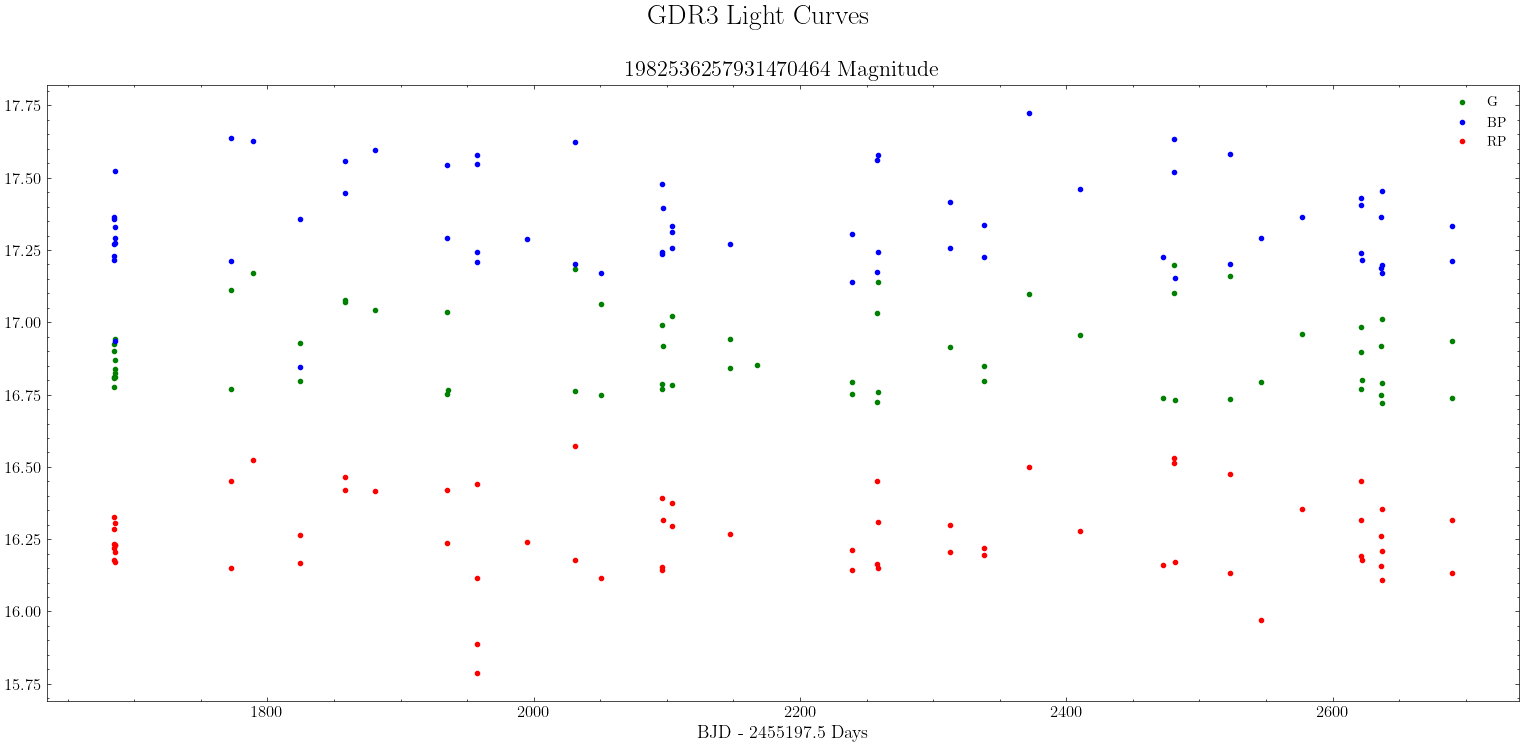
\includegraphics[scale=0.42]{Muestra/Secciones/Figures/GDR3-Light-Curves.png}

	\caption{Magnitud de \atoObjId registrada en la base de datos de Gaia DR3.
	Se puede apreciar la variabilidad de aproximadamente 0.5 mag en el brillo
	del sistema, la cual la atribuimos a la presencia de eclipses en el sistema
	binario. \citet{gdr3ReleaseDocumentation}}
	\label{gdr3AtoObjLightCurves}
\end{figure}

\subsection{Datos de ZTF}